%% cycle5_ar_tr.tex
%
%  Spitzer Space Telescope Cycle-5 Proposal Template
%
%  Use this template for Archival Research or
%  Theoretical Research proposals.  No style file is required.
%
%  Version 1.0    15 August 2007
%
%%%  For Spitzer proposal preparation resources please visit 
%    the proposal kit web page: 
%
%%%  http://ssc.spitzer.caltech.edu/propkit/ 
%
%  **In particular, please read the Cycle-5 Call for Proposals (CP).
%  **It is the definitive document that describes the requirements
%  **necessary for your proposal. THERE ARE SUBSTANTIAL
%    CHANGES TO THE ARCHIVE/THEORY PROGRAM FOR CYCLE-5.
%
%   For Cycle-5, AR and TR proposal must identify and request a specific
%   amount in one of the following $25,000 increments:
%
%  $25,000  $50,000  $75,000  $100,000  $125,000  $150,000
%
%  Proposals requesting funds outside of these amounts will not be forwarded
%  to the review panels. They will be rejected outright.
%
%  Details budgets are not longer required.
%
%    Please address all questions regarding the proposal 
%    and observation to the Helpdesk at 
%
%%%  help@spitzer.caltech.edu
%
%
%
%%%%%%%%%%%%%%%%%%%%%%%%%%%%%%%%%%%%%%%%%%%%%%%%%%%%%%%%%%%%%%%%%%%%%%%%
%
%  The template begins here.  The font must be 12 point and the margins
%  must be at least 1-inch on all sides. 
%  Don't override this.  
%
% If you compile this and find that the text is "mushed up against
% the top of the page", the default paper size for your installation 
% of latex is A4.  In order to override this, do:
% > latex texfile # where the manuscript is in a file named texfile.tex
% > dvips -Ppdf -t letter -o texfile.ps texfile
% finally, to get nice (non-blurry, searchable) pdf do:
% > ps2pdf13 texfile.ps  texfile.pdf
% if you do not have ps2pdf13, please ask your sysadmin to install it.

\documentclass[letterpaper,12pt]{article}
\usepackage{subfig,epsfig,colortbl,graphics,graphicx}
\textwidth=6.5in
\textheight=9.5in
\topmargin=-0.75in
\oddsidemargin=0.0in
\evensidemargin=0.0in

\def\lae{\mathrel{<\kern-1.0em\lower0.9ex\hbox{$\sim$}}}  
\def\gae{\mathrel{>\kern-1.0em\lower0.9ex\hbox{$\sim$}}}  
\def\msun{\ifmmode{\ {\rm M}_\odot}\else{$ {\rm M}_\odot$}\fi}  
\def\msunyr{\ifmmode{\msun \ {\rm yr}^{-1}}\else{$\msun \ {\rm 
yr}^{-1}$}\fi}  

\pagestyle{myheadings}

% Please update the following line with the title of your proposal
% and your Author name (with "et al." if more than two authors).

\markright{Spitzer Archival Studies of BCGs in X-ray Luminous Clusters, Donahue et al.}
\pagenumbering{arabic}

\begin{document}

\section{Scientific Justification}

It is becoming increasingly apparent that feedback from active nuclei
(AGN) shapes the development of clusters of galaxies (e.g. McNamara \& Nulsen 2007).  
These are the largest virialized structures in the universe, and most of their
baryons are contained in the intracluster medium (ICM), a hot, X-ray
emitting gas.  The hot gas has
1-3 keV more energy per particle than expected from virial heating in
a collapse governed by gravity alone (Wu et al. 2000; Markevitch 1998).  
The excess is larger than
can be accounted for from processes such as starburst-driven winds
during the early stages of cluster development.  

In another puzzle, recent X-ray observations by Chandra and XMM of
``cooling flow'' clusters have shown that cooling of the intracluster
gas occurs at much lower rates than predicted by simple cooling models
(e.g. Peterson et al. 2003).  This is true even in clusters with plunging central temperature
profiles and central cooling times less than 1 Gyr.  Observed cooling
rates, based on recent star formation, are only about 10\% of the
maximal, uncompensated cooling values.

Both of these puzzles may be explained by another recent X-ray
discovery.  Chandra has found giant cavities in the hot gas
surrounding nearly two dozen groups and galaxy clusters (e.g. McNamara et al. 2000;
Birzan et al. 2004).  The
cavities were carved by AGN-driven radio-emitting jets emanating from
giant cD galaxies located at their centers.  In several clusters, the
cavity systems are known to be surrounded by weak but energetic shock
fronts (eg., Forman et al. 2007).  The energy associated with the cavities and shocks
scales in proportion to the X-ray luminosity of the cluster core, and
is sufficient to quench cooling in roughly half of the systems studied
(Birzan et al. 2004).  Simultaneously, the shocks will increase the entropy of the hot
gas.  
 
These properties, combined with the existence of very short central
cooling times in the hot gas, suggest a feedback cycle of cooling, star
formation, and accretion onto the AGN, followed by relativistic jet
outbursts that heat the gas and quench cooling.  The cycle repeats on a
timescale of $10-100$ Myr (Birzan et al. 2004; Voit \& Donahue 2005). 
% This mechanism, which involves
%simultaneously building in a self-regulated fashion a supermassive
%black hole (SMBH) and the stars surrounding it, is a possible
%explanation of the well-known relation between SMBH masses and the
%properties of their bulge stellar populations (Ferrarese \& Merritt 2000; Gebhardt et al 2000). 
% THIS RADIO MODE ISN'T EXPECTED TO LEAD TO MUCH BH-BUILDING

\vspace{0.5cm}\noindent$\bullet${\sc Supergiant Cavities and Shocks in Clusters}

%%%  CITATION NUMBERS CHANGED

McNamara et al. (2005) found the most dramatic example of AGN-driven feedback in
the galaxy cluster MS0735.6+7421.  The shock energy inferred 
is $\sim 6\times 10^{61}$ erg, and the age of the shock, based on its
size and strength (Mach 1.4), is $1.04 \times 10^8$ yr. The strength of the
outburst in MS0735 implies that its $\sim 10^9\msun$ SMBH must have
accreted $\sim 3\times 10^8~\msun$ of matter in less than 100 Myr (McNamara et al. 2005).
This enormous outburst, the largest yet detected, contains enough
energy to quench a cooling flow for several Gyr.  In addition
it can provide up to $\sim 1/3$ keV per particle
of heat to the gaseous atmosphere, a substantial fraction
of the $\sim 1-3$ keV per particle of excess energy required
to ``preheat'' the cluster.  Other energetic outbursts were found 
in the Hydra A and Hercules A clusters (Nulsen et al 2005ab).  These systems show 
that powerful outbursts in clusters
are not uncommon and are likely to be energetically important
on large scales.  


\vspace{0.5cm}\noindent$\bullet${\sc Infrared Probes of the ICM Feedback Cycle}

Infrared observations are important for
studying several phases of the ICM/AGN feedback cycle.  During the
inflow phase, large amounts of cool intracluster gas are deposited on
the brightest cluster galaxy (BCG).  Signatures of this material have
been detected in the form of nebular line emission ($10^4$ K), 2 micron
molecular hydrogen emission ($\sim 10^3$ K, e.g. Donahue et al. 2000), neutral hydrogen
absorption ($10^2$ K), millimeter wavelength emission from $\sim 30$ K
molecular gas (Edge et al. 2002), and strong infrared emission at 60 and 100 microns,
presumably emitted by cool dust (e.g. Donahue \& Voit 2004).  In addition, many BCGs are
experiencing starbursts with star formation rates $\gae 10 \msunyr$ (e.g. Donahue
et al. 2007; Quillen et al. 2007),
as judged by optical-UV emission line and continuum indicators.  In
the most extreme cases, infrared luminosities are comparable to those of the
ultraluminous infrared galaxies (ULIRGS).  

%% [12] is a new citation

Owing to the surrounding cool material, some or all parts of a
bright AGN may be concealed by dust.  The eruption of the radio
jets through the dense inner gaseous atmosphere may again induce star
formation, and much of this process may likewise be hidden at short
wavelengths.  

Mid infrared spectroscopy and photometry with Spitzer can provide insights on the
feedback cycle not possible in other bands.  They will help eliminate the
dust extinction effects that we know are present in the deposition
region and provide better estimates of star formation rates and gas
ionization states.  It offers good diagnostics to distinguish between
ionization by massive stars and the presence of a luminous AGN.  Study
of the correlation between bright X-ray filaments and IR emission can
test the idea that grains provide an alternative IR cooling channel
for the hot gas.  Mid-IR spectra provide the best information on
the properties of the dust grains in BCGs and hence their origin.
Dust found in hot gas may be depleted of small grains by sputtering. 
Alternatively, dust could
be created by intermediate-age, metal-rich stars
in the BCGs or be stripped from merging satellite galaxies. Broad-band
SEDs from MIPS and IRAC observations 
allow us to estimate stellar masses, assess the contribution of AGN, and
detect excess emission from warm dust.



\smallskip

\noindent {\it What powers infrared emission from the cores of 
such clusters?}  We know that cooling flows are often very luminous in
the infrared.  However, the IRAS and ISO spatial resolutions were too
coarse to pin down the origin of the emission.  If dust acts as a major
coolant for the intracluster gas, we expect a distributed mid-IR
source.  On the other hand, if the emission is powered by a
starburst or an AGN, it should trace the more concentrated bright
regions in the CDG center.

\smallskip

\noindent {\it What are the star formation rates, and how do they compare to the
X-ray cooling rates?}   
Star formation in such objects is largely obscured by dust.  
Infrared radiation longward of $\sim 2 \mu$,
particularly from the PAH 7.7$\mu$ emission  emerging from the
dusty starbursts will provide independent star formation estimates and
help place stronger limits on the amount of gas that is actually
cooling and accreting.  The star formation rates combined with the
molecular gas masses and limits yield a total deposition rate that
can be compared to the intracluster cooling rates estimated from
XMM-{\it Newton} and {\it Chandra}.

\smallskip

\noindent {\it What are the physical conditions in the central
regions?} Using spectral line diagnostics (Voit 1992) we will determine the
ionization level and the degree of obscuration and dust content in the
central regions.  The dust content reflects abundances and the prior
physical history of the gas.  Mid-IR molecular features are important
diagnostics for the character and chemical composition of the grains.
The mid-IR neon features discriminate well between photoionization by
starlight or that by more energetic sources such as as an AGN or X-ray
emission from cooling gas [14].  The [Ne V]/[Ne III] ratio should be
small if the emission is dominated by a starburst.  In the absence of
[Ne V], the [Ne III]/[Ne II] ratio will establish the temperature of
the photoionizing stars, which is important to determining the age of
the young population and therefore the star formation rate one
infers.  A better understanding of the massive star population will
help us evaluate the effect of supernova explosions on the gas
dynamics of the CDG core.

\smallskip

Spitzer observations of these remarkable environments have broad
implications. The physics of cooling, accretion, star formation, AGN
fueling, and energy feedback forms the bedrock on which most
theoretical models for galaxy and supermassive black hole formation
are built.  The ICM feedback cycle produces one of the few
environments in the local universe where such models can be directly
tested.  

\vspace{0.5cm}\noindent$\bullet${\sc What have we learned so far?}

Broad-brand Spitzer photometry of a sample of 63 H$\alpha$-luminous BCGs
has shown a wide variety of 3-160 micron spectra, ranging from spectral energy
distributions (SEDs) with
starburst signatures (70 micron excesses, in particular) to SEDs with a mix
of AGN and starburst evidence (Quillen et al. 2007).  Starlight provides  most of the
radiant energy (Donahue et al. 2007; Figure 1). This dominance ($\sim 10^{12} L_\odot$) 
is not surprising since these BCGs are among the most massive galaxies in the universe.
The mid-IR excess appears to be typical of that generated by dust heated by the
formation of massive stars. However, the temperature of this warm dust may differ from system
to system, since we note that the peak of the emission in the more extreme galaxies studied by
Egami et al. (2006) occurs at a longer wavelength than the peak for Abell 2597 (Donahue et al. 2007).

IRS spectra for H$\alpha$-luminous
BCGs have provided further insights. A sample of 8 BCGs was studied by de Messieres et al. (2007 AAS, PI R. O'Connell;
Figure 2).
They found that some of the spectra of the BCGs are quite unlike those of normal starbursts
and AGN. One very interesting result is that most of them lack strong PAH features. 
What this could mean is that the IR-emitting dust may lack tiny grains. One plausible
reason for this lack is X-ray processing of the grains (Voit 1992). Grain sputtering (Draine \& Salpeter 1979)
by hot electrons can remove the smallest grains. However, a couple of the BCGs in the
sample do exhibit PAH features. Another unusual result is the combination of ubiquitous,
bright H$_2$ and low-ionization atomic lines together with flat continua, or even
continua that rise to the short wavelengths. 

\vspace{0.5cm}\noindent$\bullet${\sc Perspectives from ICM Entropy in Galaxy Formation Feedback}

We plan to analyze all available Spitzer data for BCGs, from IRAC and MIPS photometry to 
IRS spectroscopy in order to assess the mid-IR properties of the BCG and then compare those
properties with the more global properties of the cluster itself (X-ray luminosity, X-ray
temperature and temperature profile, and X-ray entropy distribution.) 
We have been conducting an extensive Chandra archival study of the entropy distribution in
the hot ICM of nearby clusters of galaxies (Donahue et al. 2006; Cavagnolo, PhD Thesis). We 
have now produced temperature and entropy profiles for over 140 clusters of galaxies.

Entropy is an extremely useful thermodynamic observable for studying feedback. With X-ray observations, we can 
study the distribution of entropy in the ICM by measuring $kT_x / n_e^{2/3}$ as function of position
in the cluster. The entropy distribution traces past feedback because high entropy
gas retains the imprint of any past feedback event for a very long time. 
Therefore, instead of organizing our cluster sample  by cluster luminosities and temperatures, we 
study ICM feedback through studying cluster 
entropy distributions. We can assess both current and past physical processes 
that have directly to do with feedback to the ICM, including the AGN stabilization of cool cores
(Voit \& Donahue 2005).


\section{Technical Plan}

\subsection{Sample Selection}

Ken Cavagnolo (MSU) has been completing a PhD thesis analyzing over 140
gas entropy profiles in X-ray clusters of galaxies. The data were obtained
from the Chandra archive. This work represents the largest uniform measurement
of gas entropy distributions in luminous X-ray clusters. 

We have cross-correlated this sample of well-studied X-ray clusters with
the Spitzer archive. We have identified over 90 cluster centers that have
been observed with at least one Spitzer instrument. Figure 3 summarizes our
results for the full sample. Of 143 clusters, we found MIPS observations for
77, IRAC observations for 54, and IRS observations for 33. Not all of these
observations are yet public, but they will go public sometime in 2008. 
Each one of these clusters
has accurate X-ray properties determined from Chandra data. We note that a
wide range of clusters have been observed to date, with a range of cluster
X-ray luminosities, temperatures, central entropies, and state of 
relaxation (or merger). (See figures 3-6).

We will use the standard pipeline projects to create the mosaics we need to
achieve our scientific goals. The 70-micron mosaics in our experience occasionally
require more work, beyond the standard pipeline choices, to improve the signal to noise.
However, the MOPEX GUI has proved to be a very useful tool in our previous Spitzer
work, and we plan to make good use of that. We use standard IRAF and IDL tools to
measure noise and make photometric estimates. We also use MOPEX to determine PSF-corrected
photometry as necessary. 

We already have (hard-won) experience in assembling and matching IRS spectra using
CUBISM. When possible, compare our results with any existing published results of spectra.


\subsection{Statement of Work and Schedule}


The plan of work includes:
\begin{enumerate}
\item Divide the project into IRS and MIPS+IRAC efforts.
\item For each effort, download and organize all desired Spitzer data. We will
produce a database to manage the catalog and the reduction and analysis state
for each BCG.
\item Identify systems with complex cores. These would include the cores with merging
galaxies, or cluster centers with no obvious BCG at all. These systems are the minority
of cluster centers, but will require extra work to manage.
\item Extract broad-band SEDs and IRS spectra, including observational errors.
\item Extract broad-band magnitudes from 2MASS, and, where available, Sloan Digital Sky Survey. 
Both 2MASS and SDSS magnitudes for low-redshift BCGs will need to be measured manually, since
cataloged measurements are likely to underestimate the total luminosity of the optical system.
\item Assess total IR luminosities, identify excesses in the mid-IR and the two long-wavelength
channels of IRAC (where line emission and PAHs can contribute), and total stellar luminosities.
\item Compare the X-ray properties (particularly central entropy) with the IR properties. 
One prediction we can test is that clusters in our sample with high central entropies will be much 
less likely to exhibit luminous 70-micron emission or AGN evidence. A strong prediction, based
on the assertion that low-entropy gas feeds both star formation and AGN activity, is that
none of the high-central entropy systems will.
\end{enumerate}

We are requesting \$100,000 total. \$75,000 will go to MSU to support 5 months of a 
postdoc and 1 month of summer salary for the PI Megan Donahue. Donahue and the postdoc
will lead the MIPS and IRAC analysis, and some of the IRS work. This amount will also include
support for 2 domestic trips for the postdoc, computer support (such as an external 
disk drive, software IDL license renewals - a shared cost), and publications.
\$25,000 will go to the University of Virginia to support the IRS work
of a graduate student, utilizing CUBISM under the direction of Prof. O'Connell.

\section{Figures and Tables}
\begin{figure}[t]
  \centering
  \subfloat[]{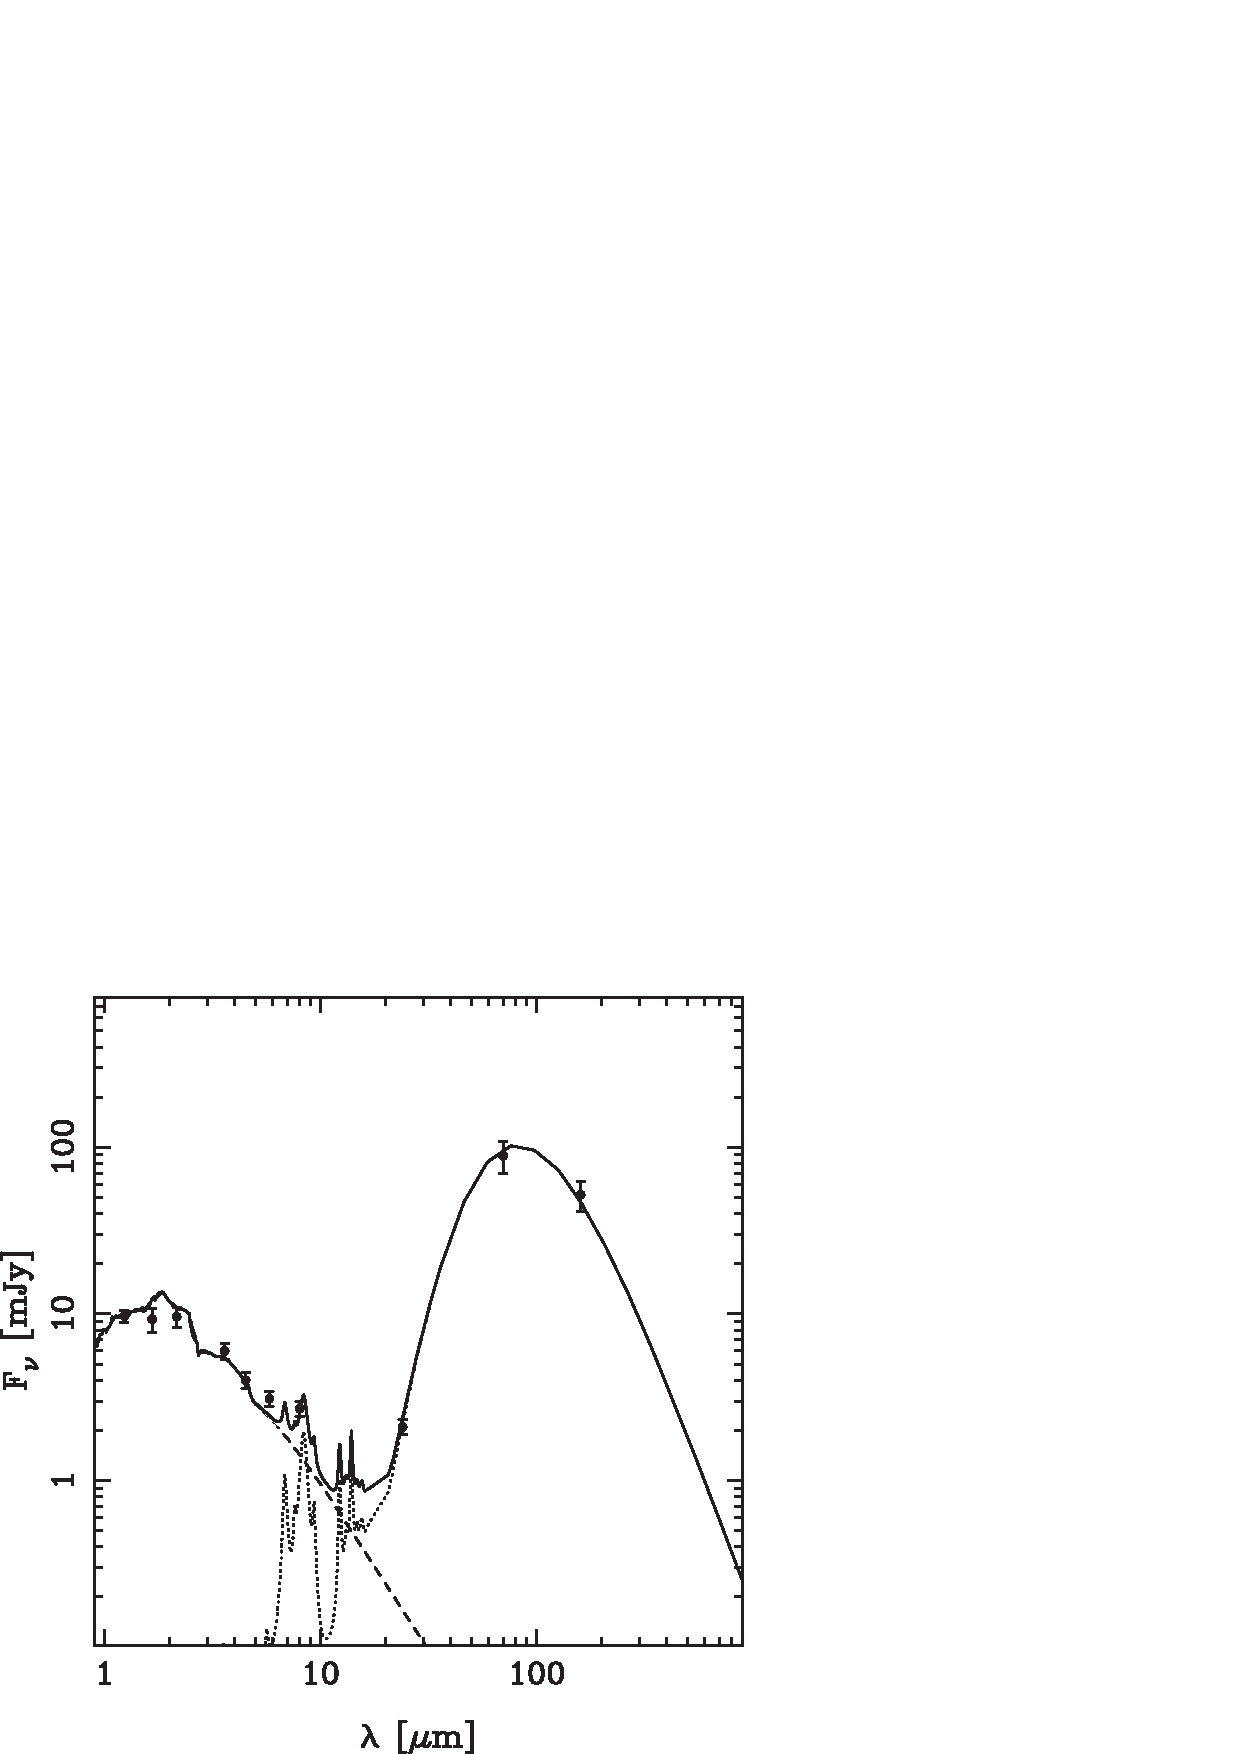
\includegraphics[height=0.45\textheight]{Spitzer_SED_A2597}}
  \subfloat[]{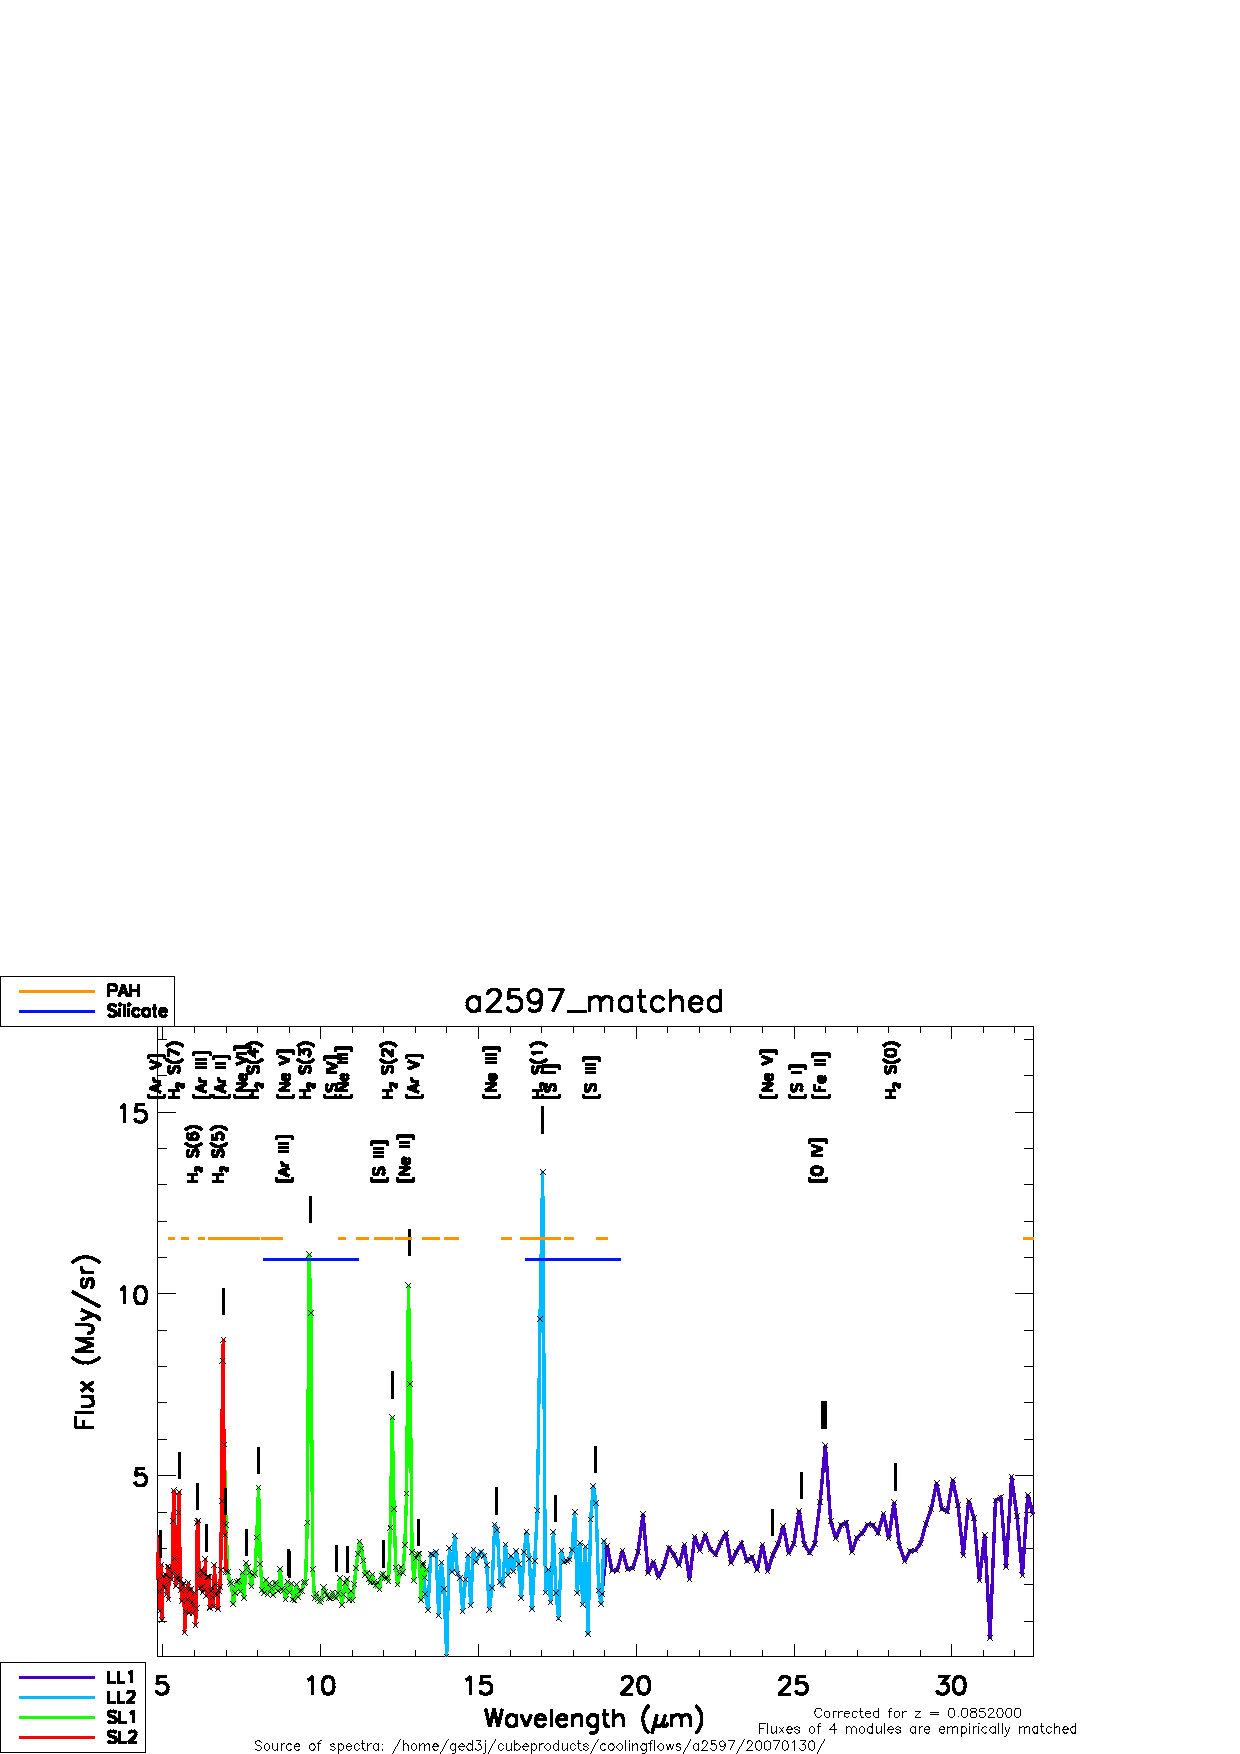
\includegraphics[height=0.45\textheight]{a2597_matched}}
  \caption{\small
           {\bf a)} SED for the BCG in Abell 2597 from IRAC
            and MIPS photometry (Donahue et al. 2007). 
           {\bf b)} IRS spectrum for the BCG in Abell 2597. Note the
            prominent H$_2$ lines and lack of PAH features
            (deMessieres et al. 2008).}
\end{figure}

\clearpage
\begin{figure}[t]
    \begin{minipage}[t]{0.5\linewidth}
        \centering
        \includegraphics*[width=\textwidth, trim=28mm 10mm 30mm 17mm, clip]{spitzer_k0}
        \caption{\small This figure shows the central entropy (in units of keV cm$^2$) for 143
        Chandra clusters. Cluster centers with MIPS observations are
        plotted with red squares; IRAC observations have blue circles; IRS
        observations green triangles. There is excellent overlap in parameter
        space between the Spitzer and the Chandra archive samples, except for
        $z<0.1$, $K_0>10$ keV cm$^2$ (for which we are also submitting an
        observing proposal.)} 
        \label{fig:figure1}
    \end{minipage}
    \hspace{0.25cm}
    \begin{minipage}[t]{0.5\linewidth}
        \centering
        \includegraphics*[width=\textwidth, trim=28mm 10mm 30mm 17mm, clip]{spitzer_hak0}
        \caption{\small Same code as for Figure \ref{fig:figure1}, but for the 75 clusters for which we also have
        H$\alpha$ measurements. Note that there has been excellent Spitzer coverage of
        these systems, to some extent owing to O'Dea's project for luminous
        H$\alpha$ systems, but also because these were thought, prior to launch, to be
        the best bets for bright IR emission.}
        \label{fig:figure2}
    \end{minipage}
\end{figure}

\begin{figure}[t]
    \begin{minipage}[t]{0.5\linewidth}
        \centering
        \includegraphics*[width=\textwidth, trim=28mm 10mm 30mm 17mm, clip]{spitzer_lx}
        \caption{\small Archived Spitzer observations of cluster centers presented for
        X-ray luminosity (bolometric) vs. redshift. Coding the same as Figure \ref{fig:figure1}.}
        \label{fig:figure6}
    \end{minipage}
    \hspace{0.25cm}
    \begin{minipage}[t]{0.5\linewidth}
        \centering
        \includegraphics*[width=\textwidth, trim=22mm 8mm 30mm 15mm, clip]{splots}
        \caption{\small Entropy profiles for 143 clusters of galaxies. (Cavagnolo 2008
        PhD Thesis). Note that nearly all of the clusters have the same entropy at 
        100-200 kpc, but there is a wide range of central entropy, or equivalently,
        central cooling times. The clusters with low central entropy, or short 
        radiative cooling times also are clusters with cool cores and strong 
        metallicity (iron) abundance gradients.}
        \label{fig:figure4}
    \end{minipage}
\end{figure}

\clearpage
\section{References}
Birzan, L. et al. 2004, ApJ, 607, 800. \\
Donahue, M. et al. 2000, ApJ, 545, 670. \\
Donahue, M. et al. 2007, ApJ, in press (arXiv:0708.1427). \\
Donahue, M. \& Voit, G. M. 2004, Carnegie Centennial Review, arXiv:astro-ph/0308006. \\
Draine, B. T.\& Salpeter, E. E. 1979, ApJ, 231, 77.
%Ferrarese \& Merritt 2000, ApJ, 539, L9
Edge, A. et al. 2002, MNRAS, 337, 63. \\
Egami, E. et al. 2006, ApJ, 647, 922. \\
Forman, W. et al. 2007, ApJ, 665, 1057. \\
%Gebhardt et al. 2000, ApJ, 539, L13. \\
Markevitch, M. 1998, ApJ, 504, 27. \\
McNamara, B. R. \& Nulsen, P. E. J. 2007, ARAA, 45, 117.\\
McNamara, B.R. et al. 2000, ApJ, 534, L135. \\
McNamara, B.R., et al. 2005, {Nature}, 433, 45. \\
Nulsen, P. E. J. et al. 2005ab: ApJ 625, L9; ApJ 628, 629.\\
Peterson, J.R. et al. 2003,ApJ, 590, 207. \\
Quillen, A. et al. 2007, ApJS, in press. (arXiv: 0711.1118). \\
Voit, G. M. \& Donahue, M. 2005, ApJ, 634, 955. \\
Voit, G. M. 1992, ApJ, 399, 495.\\
Voit, G. M. 1992, MNRAS, 258, 841.\\
Voit, G. M, Donahue, M. 2005, ApJ, 634, 955. \\
Wu, K.K.S. et al. 2000, MNRAS, 318, 889. \\


\section{Brief Resume/Bibliography}

The PI Megan Donahue is an associate professor in the department
of Physics and Astronomy at Michigan State University. She
has 25 years of multi-wavelength observing experience 
from the mid-infrared to the X-rays, including near-IR imaging, optical 
spectroscopy and imaging, UV spectroscopy. She has also published theory papers
in the area of the physical gas and radiation processes in the IGM and ICM.
Her current main research interests are the formation and evolution of galaxies and clusters,
and in cluster cosmology. She has published 57 refereed journal articles on
these topics, and is a co-author of The Cosmic Perspective, one of the 
most popular astronomy textbook for undergrads on the market. 

Co-I G. Mark Voit is an associate professor in the department
of Physics and Astronomy at Michigan State University, and his specialty
is theoretical astrophysics. His areas of expertise are cosmology, 
gas and dust processes, clusters of galaxies, AGN. He works extensively with
simulations of galaxy and cluster formation to produce observable predictions
at the X-ray, optical, and infrared wavelengths. He is also a co-author of the
Cosmic Perspective.

Co-I Ken Cavagnolo is an MSU graduate student entering his final year. He has 
extensive X-ray data analysis experience, including the analysis of 200 Chandra
cluster observations. He plans to expand his data analysis skills to include 
Spitzer with projects proposed for this observing cycle.

Co-I Robert O'Connell is a professor in the department of Astronomy at 
the University of Virginia. He is an expert in UV and spectral diagnostics
of stellar populations and emission line systems in elliptical galaxies,
merger systems, globular clusters.

PI Relevant publications:

Quillen, A. et al. 2007, ApJS, accepted. (astro-ph/0711.1118): An infrared survey
of the brightest cluster galaxies: Paper I. (Paper II, O'Dea et al. will be reviewed 
by the time this proposal is reviewed.)

Donahue, M. et al. 2007, ApJ, accepted (astro-ph/0708.1427): Infrared Emission from the 
nearby cool core cluster Abell 2597

Donahue, M. et al. 2007, AJ, 134, 14. Star Formation, Radio Sources, Cooling X-ray Gas
and Interactions in the Brightest Cluster Galaxy in 2A0335+096.

Sun, M., Donahue, M., Voit G. M. 2007, ApJ, accepted. H-alpha tail, intracluster HII regions,
and star formation: ESO-137 in Abell 3667.

Donahue, M. et al. 2006, ApJ, 643, 730. Entropy profiles in the cores of cooling flow 
clusters of galaxies.

Voit, G. M. \& Donahue, M. 2005, ApJ, 634, 955. An observationally motivated framework
for AGN heating of cluster cores

Donahue, M. et al. 2005, ApJ, 630, L13. Two clusters of galaxies with radio quiet cooling cores.




\section{Status of Existing Spitzer Programs}

The PI has not been a PI of a previous Spitzer program.

Donahue, M. et al. 2007, ApJ is based on data from a Spitzer GO program, PI W. Sparks.

Robert O'Connell in PI on Spitzer program P3384, "Mid-Infrared
Spectroscopy of Massive Cluster Cooling Flows," and is a principal Co-I
on Spitzer program 20345, "Starbursts and Supercavities in Clusters of
Galaxies."  The datasets from these programs have been combined.  We
had considerable difficulty with early reduction of the IRS spectral
mapping data but with the advent of CUBISM have obtained excellent
extractions for all targets.  

Publication: de Messieres, G., O'Connell, R.W., Donahue, M., McNamara,
B.R., Nulsen, P.E.J., Voit, M., \& Wise, M.W. 2008, "Spitzer
Mid-Infrared Spectra of Selected Galaxy Cluster Cooling Flows," BAAS,
vol 40. 


\end{document}
